\chapter{Architecture}
\label{sec:architecture}
\minitoc
\vspace*{1cm}

This chapter illustrates the general design of the fuzzer without getting into too much implementation details. The in-depth breakdown of the fuzzer's components is more thoroughly described in Chapter ~\ref{sec:implementation}. The key components that will be elaborated here are the high-level working view of \pname{}, instrumentation although its details are out of the scope of this thesis, 

\section{A Fuzzing Session}
A regular fuzzing session using \pname{} can be seen at Figure ~\ref{sec:architecture}. It displays the process from the point the request is sent up to the point where a response is received. A request may be produce in one of two ways; it can be a mutated form of a previously made request which turned out to be interesting or as a new link that has been discovered by the in-built crawler but has not been visited yet. When the response is received, it is parsed in order to extract the execution time, vulnerabilities it may triggered, coverage score, and record newly discovered links.


\begin{figure}[ht]
 \centering
 \captionsetup{justification=centering}
 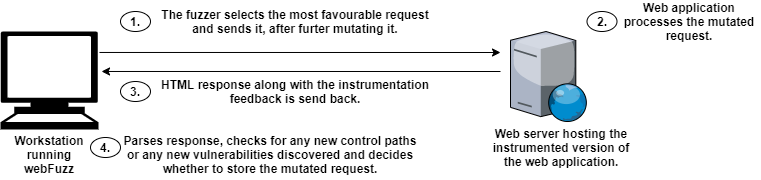
\includegraphics[width=5.0in]{figures/architecture.png}
 \caption{Simplified work process of \pname{}.}
 \label{fig:architecture}
\end{figure}

\section{Mutations}
In most cases sending randomly generated inputs will be quickly rejected by the target program as the data is syntactically invalid. One way to increase our chances of obtaining valid input is through mutational fuzzing where small modifications are made to existing inputs that may still keep the input valid, yet exercise new behaviour. For creating fuzz test cases, mutation is an essential part of the fuzzing process. It is vital because we need it to maintain diversity in our test cases in order to avoid stagnation on a suboptimal plateau in the search space ~\cite{seal2016Genetic}. Choosing which mutation function to use in order to detect the most vulnerabilities, is both a challenging and empirical task. If changes made to the input are to conservative, only a limited code coverage will be achieved as there may not be enough to trigger new control flows whereas too aggressive tweaks can destroy much of the input data structure and lead to the test cases failing at an early stage of the execution ~\cite{zalewski2014Mutations}.

\pname{} currently supports five kinds of mutation functions, although the tool can be easily
extended to support custom GET or POST parameter mutations. The mutation functions it employs are injection of known XSS payloads, mixing the parameters from other requests (cross-over), insertion of a randomly generated payload, insertion of syntax aware payloads and altering the
parameter types. Some parameters may get randomly opted out from the mutation process too. This can be useful in cases where certain parameters need to remain unchanged for certain areas of the program to execute. Regarding the known XSS payloads, unlike many fuzzers that employ malicious payload generation via the use of a specific grammar, \pname{} chooses randomly from a corpus that consists of real-life XSS payloads. The corpus was created with payloads that where found scattered all over the internet, in open-source repositories mainly ~\cite{xsspayloadfirst,xsspayloadsecond}. Such payloads may get further mutated by prepending or appending to them random strings or specific HTML, JavaScript and PHP syntax tokens.

\section{Detecting Vulnerabilities}
\pname{} is able to detect Reflected and Stored Cross-Site Scripting(XSS) vulnerabilities, and subsequently, web applications that can be exploited for Distributed Denial of Service (DDoS) attacks. In order to detect the aforementioned vulnerabilities, we do a string-matching for the injected, possibly malicious, payload in the returned HTML response. This method may be the most efficient in terms of speed, however, it can result in high number of false positives, as the location of the payload in the response is not accounted for. False positives arise when the tool reports that an XSS was detected when in fact it was not one. One example of this would be if the XSS payload is returned enclosed with double quotes inside an HTML element's attribute. If the web application correctly escapes any double quotes found in the XSS payload then the payload will not be executable. There are plans to improve the efficiency of our XSS detection method which are discussed in Chapter ~\ref{sec:futurework}.

% NEW SECTION
\section{Mutation}

\section{Automated Vulnerability Addition}
